% ============================================================================
% Section 5: Preliminary results  (replaces the empty Section 5 of the midterm)
% Needs: \usepackage{booktabs,graphicx}. Put fig_dsrl_small.pdf and fig_dsrl_full.pdf next to main.tex.
% Every number below comes from results/*.json, runs/dsrl_small_eideas3/ or runs/dsrl_full_eideas3/.
% ============================================================================
\section{Preliminary results}

We report four completed pieces of evidence: closed-loop performance of the
frozen Flow BC policies, numerical checks of the flow interface used for value
estimation, a staged pilot of a DSRL-style latent-steering learner on Can, and
full-budget latent-steering runs on all three tasks.
The Q-gating comparison (conditions B and C in Table~2) is implemented but has
not yet been run, so no gating result is reported here.

\subsection{Frozen Flow BC}

Each task was trained once (seed 0, 10{,}000 updates) and evaluated with the
policy frozen on 20 reset seeds (30000--30019). Table~\ref{tab:bc} reports the
results. Lift and Can succeed in 12 of 20 episodes; Square succeeds in 3 of 20.
With 20 episodes, the 95\% Wilson intervals are wide and overlap substantially
for Lift and Can. On Lift, the final validation loss (0.955) is far above the
training loss (0.203), consistent with overfitting its 36 training
demonstrations; Can and Square show no such gap. Inference costs about 3.2\,ms
per control step on a CPU, so sampling is not a bottleneck for online
learning.

\begin{table}[t]
  \centering
  \small
  \caption{Frozen Flow BC, one training seed, 20 evaluation episodes per task.}
  \label{tab:bc}
  \begin{tabular}{lrrrrr}
    \toprule
    Task & Success & 95\% Wilson CI & Train / valid loss & Eval.\ steps & ms / step \\
    \midrule
    Lift   & 12/20 (60\%) & [0.39, 0.78] & 0.203 / 0.955 & 3{,}007 & 3.29 \\
    Can    & 12/20 (60\%) & [0.39, 0.78] & 0.510 / 0.480 & 3{,}758 & 3.18 \\
    Square &  3/20 (15\%) & [0.05, 0.36] & 0.377 / 0.457 & 8{,}971 & 3.22 \\
    \bottomrule
  \end{tabular}
\end{table}

\subsection{Numerical checks of the flow interface}

Value estimation and latent steering both rely on mapping between Gaussian noise
and arm commands through the trained flow. For eight fixed states per task, we
decoded seeded noise to an action and encoded it back. The maximum
per-coordinate round-trip error falls from $2.0\times10^{-4}$ (Lift),
$6.5\times10^{-5}$ (Can) and $9.0\times10^{-5}$ (Square) at 16 RK4 steps to below
$2.0\times10^{-7}$ at 64 steps, so integration error is small at the default
step count. All 17 unit tests pass on the GPU machine, including tests that
check that float64 learner updates on CUDA match the CPU. On a synthetic two-mode flow, where
only one mode is rewarded, latent steering raises the rewarded-mode fraction
from 0.506 under BC to 0.99, which confirms that the learner can redirect a
frozen generator. This synthetic check is not a robotics result.

\subsection{Latent-steering pilot on Can}

As a lower-cost route to online improvement, we implemented a DSRL-inspired
learner~[8] that keeps the flow frozen and learns a Gaussian policy over its
input noise. An action critic is trained on executed transitions, a noise critic
is distilled from it through the frozen decoder, and a KL penalty with weight
$\beta$ keeps the noise policy near the Gaussian prior. We ran a staged pilot on
Can using two RTX~5080 GPUs. The pilot used a Can flow retrained with the
configuration and seed of Table~\ref{tab:bc}; under fixed seeds it also reaches
60\% BC success.

\begin{itemize}
  \item \textbf{Warmup (stage B).} 50 BC episodes (33 successful, 8{,}902
  transitions) seed the replay buffer. Before training, the untrained steering
  policy reproduced the BC actions exactly, which checks that the components are
  connected correctly.
  \item \textbf{Offline only (C).} 4{,}000 updates on the warmup buffer with no
  new interaction.
  \item \textbf{Online (D, E).} 5{,}000 further environment steps at 5 updates
  per step (29{,}000 updates in total), with $\beta=3$ (D) and $\beta\in\{1,10\}$
  (E). C, D and E all start from the same buffer.
\end{itemize}

Every evaluation compares BC and the steered policy on the same 20 reset
seeds (40000--40019), so the two can be compared episode by episode.
Table~\ref{tab:dsrl} and Figure~\ref{fig:dsrl} summarize the results. With
$\beta=3$, success rises from 60\% to 75\% after 5{,}000 online steps. Three
episodes were solved only by the steered policy and none only by BC. A
smaller penalty ($\beta=1$) moves further from BC and ends below it (55\%,
with 3 episodes lost and 2 gained). A larger one ($\beta=10$) barely changes
behavior (65\%, latent KL $4\times10^{-4}$). Offline training alone left
success unchanged.

These results are encouraging but not conclusive. The 95\% Wilson interval for
15/20 is [0.53, 0.89], which overlaps BC's [0.39, 0.78], and only one seed was
run. The action-critic loss (Figure~\ref{fig:dsrl}b) shows isolated
single-batch spikes of up to $\sim$50 against a late-training median of
0.7--0.8; after each spike the loss returns to its previous level at the next logged
update. Its median increases as the TD target grows in magnitude (mean target
$-17$ offline, about $-64$ online), which matches the longer return horizon
of online data. Latent standard deviations stay between 0.96 and 1.0, so the
noise policy shows no sign of collapse. Updates take 23--28\,ms on the GPU,
which put a full-budget run (100 warmup episodes, $10^5$ online steps, 20
updates per step) at an estimated 24--28\,h per task. The runs in
Section~\ref{sec:dsrl-full} took 13.6--19.6\,h.

\begin{table}[t]
  \centering
  \small
  \caption{Latent-steering pilot on Can, paired over 20 evaluation seeds. BC succeeds in 12/20 (60\%) at every evaluation.
  ``DSRL only'' and ``BC only'' count episodes solved by one policy and not the other.}
  \label{tab:dsrl}
  \begin{tabular}{llrrrr}
    \toprule
    Run & Setting & Online steps & Steered success & DSRL only & BC only \\
    \midrule
    C & offline, $\beta=3$   & 0     & 12/20 (60\%) & 1 & 1 \\
    D & online, $\beta=3$    & 2{,}500 & 12/20 (60\%) & 0 & 0 \\
      &                      & 5{,}000 & \textbf{15/20 (75\%)} & 3 & 0 \\
    E & online, $\beta=1$    & 2{,}500 & 14/20 (70\%) & 2 & 0 \\
      &                      & 5{,}000 & 11/20 (55\%) & 2 & 3 \\
    E & online, $\beta=10$   & 2{,}500 & 13/20 (65\%) & 1 & 0 \\
      &                      & 5{,}000 & 13/20 (65\%) & 1 & 0 \\
    \bottomrule
  \end{tabular}
\end{table}

\begin{figure}[t]
  \centering
  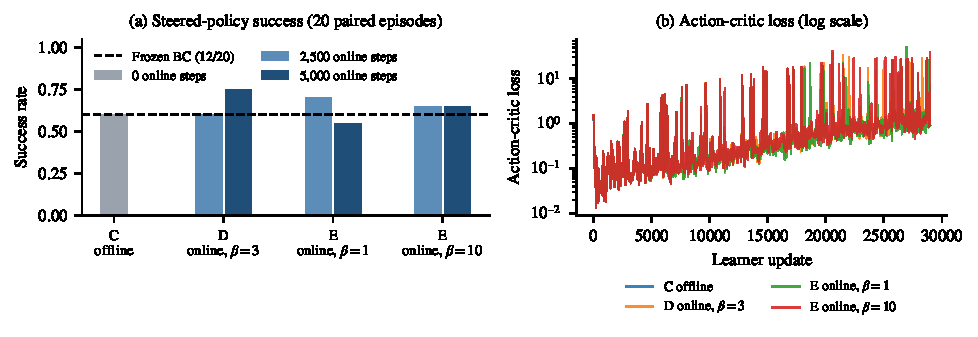
\includegraphics[width=\linewidth]{fig_dsrl_small.pdf}
  \caption{Latent-steering pilot on Can. (a) Steered-policy success at each
  evaluation; the dashed line is frozen BC on the same seeds. (b) Action-critic
  loss, logged every 50 updates.}
  \label{fig:dsrl}
\end{figure}

\subsection{Full-budget latent steering on Lift, Can, and Square}
\label{sec:dsrl-full}

After the pilot, we ran the full latent-steering budget on all three tasks with
$\beta=3$ and one training seed: 100 BC warmup episodes, then $10^5$ online
steps at 20 updates per step (2{,}001{,}500 updates). The three processes ran
concurrently, Lift on one GPU and Can and Square sharing the other, and
finished in 13.6, 17.6 and 19.6 hours, with mean update times of 22--28\,ms.
The frozen flow weights were unchanged at the end of every run. Because these
flows were retrained on the GPU workstation, BC was re-measured on the same 50
evaluation seeds (40000--40049) used for the steered policy. It succeeds in
23/50 episodes on Lift, 26/50 on Can and 4/50 on Square
(Table~\ref{tab:dsrl-full}), within the intervals of Table~\ref{tab:bc}.

\begin{table}[t]
  \centering
  \small
  \caption{Full-budget latent steering, one training seed, $\beta=3$, 50 paired
  evaluation episodes every $10^4$ online steps. Brackets are 95\% Wilson
  intervals. ``Steered only'' and ``BC only'' count episodes at the final
  evaluation solved by one policy and not the other.}
  \label{tab:dsrl-full}
  \setlength{\tabcolsep}{4pt}
  \begin{tabular}{lrrrrrrr}
    \toprule
    Task & Warmup wins & BC & Steered, $10^4$ & Steered, final & Best & Steered only & BC only \\
    \midrule
    Lift   & 51/100 & 23/50 [0.33, 0.60] & 43/50 & \textbf{46/50} [0.81, 0.97] & 48/50 & 23 & 0 \\
    Can    & 61/100 & 26/50 [0.39, 0.65] & 39/50 & \textbf{44/50} [0.76, 0.94] & 44/50 & 18 & 0 \\
    Square &  9/100 &  4/50 [0.03, 0.19] &  5/50 & 0/50 [0.00, 0.07]          &  5/50 &  0 & 4 \\
    \bottomrule
  \end{tabular}
\end{table}

On Lift and Can, latent steering improves substantially on BC. Steered success
exceeds BC at all ten evaluations on both tasks, and the final 95\% intervals do
not overlap BC's. Most of the gain appears within the first $10^4$ online steps
(86\% on Lift, 78\% on Can), followed by smaller changes
(Figure~\ref{fig:dsrl-full}a). At the final evaluation, the steered policy
solves 23 Lift and 18 Can episodes that BC fails, and loses none that BC solves.
It also finishes faster: successful episodes average 42 instead of 55 steps on
Lift and 111 instead of 119 on Can. Online training episodes show the same
trend, with 90 of the last 100 successful on Lift and 94 on Can. These are
still single-seed results, so variation across training seeds remains
unmeasured.

Square fails. With only 9 successful warmup episodes among about 47{,}000
transitions, the steered policy stays near BC (0--5/50, against BC's 4/50) for
the first 60{,}000 online steps, then solves no evaluation episode from 70{,}000
steps onward. The learner logs indicate critic divergence rather than slow
learning. Each step earns reward $-1$, or 4 on success, which ends the episode,
so every true value lies in $[-100, 4]$. Square's mean TD target leaves that
range at 1.28 million updates (about 64{,}000 online steps), falls below $-300$
by 71{,}000 steps, and ends near $-10^3$ (Figure~\ref{fig:dsrl-full}b). Its
late-training action-critic loss has a median near $10^4$, compared with 2.7 on
Can. The steering policy follows the diverged critic away from the prior. Its
median late KL is 2.4, compared with 0.014 on Can and 0.10 on Lift, its latent
means reach the $\pm2$ bound, and its smallest latent standard deviation falls
to 0.007. Lift shows a milder version of the same bias: its mean TD target
settles near $-125$, below the reachable minimum, without harming success.
Sparse successes combined with 20 updates per step appear to make the critic
unstable. Bounding TD targets to the reachable range, lowering the update
ratio, and adding demonstrations or more warmup episodes to replay are the
natural fixes.

\begin{figure}[t]
  \centering
  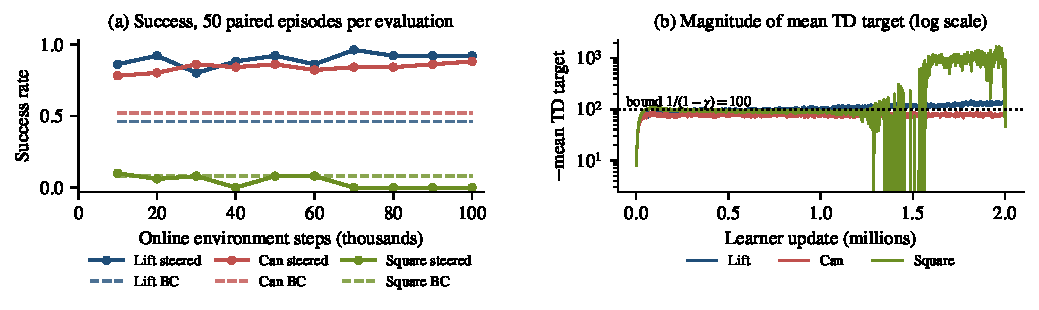
\includegraphics[width=\linewidth]{fig_dsrl_full.pdf}
  \caption{Full-budget latent steering, one training seed. (a) Steered (solid)
  and frozen BC (dashed) success at each evaluation, against online environment
  steps after warmup. (b) Magnitude of the mean TD target, logged every 100
  updates; the dotted line marks the largest magnitude any true value can
  reach.}
  \label{fig:dsrl-full}
\end{figure}
